\DeclareUnicodeCharacter{FF0C}{fi}
%=================================================================
\documentclass[journal,article,submit,moreauthors,pdftex]{Definitions/mdpi}
%=================================================================
\firstpage{1}
\makeatletter
\setcounter{page}{\@firstpage}
\makeatother
\pubvolume{xx}
\issuenum{1}
\articlenumber{5}
\pubyear{2019}
\copyrightyear{2019}
%\externaleditor{Academic Editor: name}
\history{Received: date; Accepted: date; Published: date}
%\updates{yes} % If there is an update available, un-comment this line
%=================================================================
% Full title of the paper (Capitalized)
\Title{Tip estimation method in phantoms for curved needle using 2D transverse Ultrasound images}

% Author Orchid ID: enter ID or remove command
%\newcommand{\orcidauthorA}{0000-0002-4187-8106} % Add \orcidA{} behind the author's name
%\newcommand{\orcidauthorB}{0000-0000-000-000X} % Add \orcidB{} behind the author's name

% Authors, for the paper (add full first names)
\Author{Zihao Li $^{1}$,Shuang Song $^{1,}$*, Li Liu $^{2,}$* and Max Q.-H. Meng, Fellow, IEEE $^{2,}$}

% Authors, for metadata in PDF
\AuthorNames{Zihao Li, Shuang Song, Li Liu and  Max Q.-H. Meng}

% Affiliations / Addresses (Add [1] after \address if there is only one affiliation.)
\address{$^{1}$ \quad School of Mechanical Engineering and Automation, Harbin Institute of Technology, Shenzhen 518055, China;lzh\_lejou@163.com (Z.L.);songshuang@hit.edu.cn (S.S.)\\
$^{2}$ \quad Robotics,Perception and Artificial Intelligence Lab,The Chinese University of Hong Kong, N.T., Hong Kong 999077, China;liliu@cuhk.edu.hk (L.L.);qhmeng@ee.cuhk.edu.hk (M.Q.H.M.)}

% Contact information of the corresponding author
\corres{Correspondence: songshuang@hit.edu.cn(S.S.);liliu@cuhk.edu.hk(L.L.)}

% Current address and/or shared authorship
%\firstnote{Current address: Harbin Institute of Technology (Shenzhen), Shenzhen, China, 518055}
%\secondnote{These authors contributed equally to this work.}
% The commands \thirdnote{} till \eighthnote{} are available for further notes

% Abstract (Do not insert blank lines, i.e. \\)
\abstract{Flexible needles have been widely used in minimally invasive surgeries, especially in percutaneous interventions.
Among the interventions, tip position of the curved needle is very important, since it directly affects the success of the surgeries.
In this paper, we present a method to estimate tip position of a long-curved needle by using 2D transverse Ultrasound images from a robotic ultrasound system.
Ultrasound is first used to detect the cross section of long-flexible needle.
A new imaging approach is proposed based on the selection of numbers of pixels with higher gray level, which can directly remove the lower gray level to highlight the needle.
After that, needle shape tracking method is proposed by combining the image processing with Kalman filter by using 3D needle positions, which develops a robust needle tracking procedure from 1 mm to 8 mm scan intervals.
Shape reconstruction is then achieved using curve fitting method.
Finally, the needle tip position is estimated based on the curve fitting result.
Experimental results showed that the estimation error of tip position is less than 1 mm within 4 mm scan intervals.
The advantage of the proposed method is that the shape and tip position can be estimated through scanning the needle's cross sections at intervals along the direction of needle insertion without detecting the tip.
%The advantage of the proposed method is that the tip is estimated through scanning the needle's cross sections.
%Moreover, if the needle is deflected in the tissue, the tip position can be estimated accurately when the probe scans along the direction of needle insertion.
}

% Keywords
\keyword{Needle tracking; Tip estimation; Transverse Ultrasound images; Percutaneous interventions.}

\usepackage{subfigure}
\usepackage{optidef}
%%%%%%%%%%%%%%%%%%%%%%%%%%%%%%%%%%%%%%%%%%
\begin{document}
%%%%%%%%%%%%%%%%%%%%%%%%%%%%%%%%%%%%%%%%%%
\section{Introduction}
With the help of the beveled-tip needle, percutaneous interventions and therapies have been widely involved in current clinical procedures such as brachytherapy \cite{Orlando2019,Henken2017}, tissue biopsy  \cite{Nachabe2015,Mehrjardi2017a}, and drug delivery \cite{Jun2018,Park2018}.
In interventions procedures, less needle misplacement will lead to a more reliable treatment and a more accurate medical practice. According to the clinical studies \cite{Renfrew2018,Rossa2017b}, the needle is easy to deflect, which will cause needle tip misplacement and may lead to unsafe. Due to needle-tissue interaction, improper insertion force or physiological motions such as breathing, the targets or obstacles may become unstable, which will lead to unexpected error.
To address the challenge, real-time feedback is highly required.
Usually, medical imaging devices are used, such as ultrasound (US) \cite{VandeBerg2019a}, computerized tomography (CT) \cite{Li2018,Shellikeri2017a}, or magnetic resonance imaging (MRI) \cite{Henken2017,Raj2019}.
Generally, the image-guided percutaneous interventions are conducted with the use of CT or MRI.
However, ultrasound-guided procedures are more attractive due to its advantages such as none ionizing radiations and real-time detection.

Many studies for guidance of needle during the insertion operation have been conducted with the help of ultrasound devices, and 2D ultrasound images is quite general to use, especially for the sagittal one (shown in figure \ref{fig:001}).
Elif et al proposed to use circular Hough transform to locate the needle tip accurately, even the imaging is out-of-plane \cite{Ayvali2015}.
Kaya et al. localized the needle axis and estimated the needle tip by using a Gabor Filter in sagittal US images \cite{Kaya2014}.
To execute in real time, they improved the processing time by applying the bin packing method \cite{Kaya2015}.
Recently, template-based tracking method with the efficient second order minimization optimization method has been used to track the needle \cite{Kaya2019}.
In recent studies, more and more novel ideas have been used to locate the needle and evaluate its tip in sagittal US images, such as the use of signal attenuation maps \cite{Mwikirize2018}, Convolution neural networks (CNN) \cite{Mwikirize2018a} and maximum likelihood estimation sample consensus (MLESAC) method \cite{Xu2018a}.
However, a demerit of using sagittal US images is that out-of-plane bending of the needle cannot be detected.
Therefore, the methods applied on sagittal US images are not suitable for the needle which may be deflected by the inevitable factors, especially for long needles.

\begin{figure}[H]
\centering
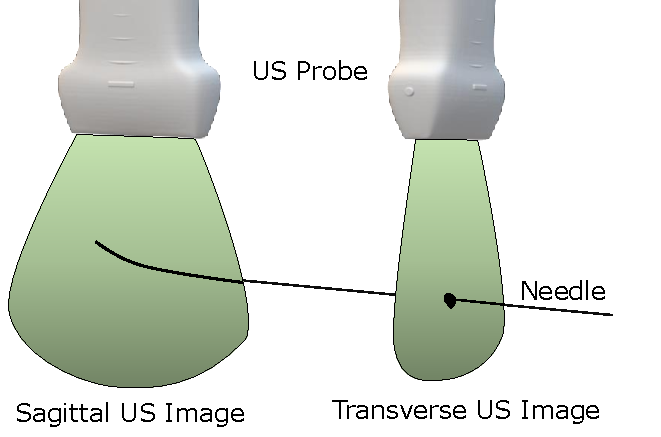
\includegraphics[width=0.5\textwidth]{figures/2/fz_1.pdf}
\captionsetup{width=12 cm,justification=centering}
\caption{Two methods by using 2D ultrasound for detection.}\label{fig:001}
\end{figure}

An alternate solution for this problem is to use 3D US image, which has been widely studied in recent researches.
Yue et al. used a RANSAC method to detect the needle in a 3D US situation and Kalman filter has been used to reduce the error \cite{Yue2012}.
Chatelain et al. used the particle filtering to track a robot-guided flexible needle by using 3D US \cite{Chatelain2015}.
In addition, a convolutional neural network with conventional image processing techniques has also been used to track and detect the needle \cite{Arif2019} and a naive Bayesian classifier was used to localize needle among 3D US volume voxels \cite{Younes2018a}.
However, the large 3D US volumetric dataset would make it difficult to obtain and process the online data.

Due to the above disadvantages, sagittal US images and 3D US volume are not suitable for a long flexible needle.
In order to locate the needle accurately, methods that using transverse US images (shown in figure \ref{fig:001}) have been used successfully in some studies.
For example, Vrooijink et al.\cite{GustaafJ.Vrooijink2013} presents a method to track the flexible needle during the insertion into a gelatin tissue by using 2D US images perpendicular to its needle tip, though the background is pure, without any noise, which seems to be experimental and impractical.
Waine et al.\cite{Waine2015b,Waine2016a,Waine2015c} focus on the research about the needle insertion, in permanent prostate brachytherapy (PPB),where needles are typically 200 mm and easily to be deflected, indicating the fact that the rectum limits the movement of US probe.
As a result, it is hard to acquire the sagittal images of curved needle to observe the deflection during needle insertion, since the sagittal method has a strong relationship to the movement of the US probe when the needle is out of the view-field of the US images, and this movement maybe deform the prostate as well as affect the needle target.
%Besides, 3D US is not suitable for the real-time detection because the difficult processing of volumetric data.
%3D US scanners are not the universal device in the majority of hospitals and clinics.
For a deflected needle, the transverse US image is a better choice for its detection.
The transverse US image is easily to be acquired when the US probe scanning along the needle, no matter how much the needle is curved, unlike sagittal images.

\begin{figure}[H]
\centering
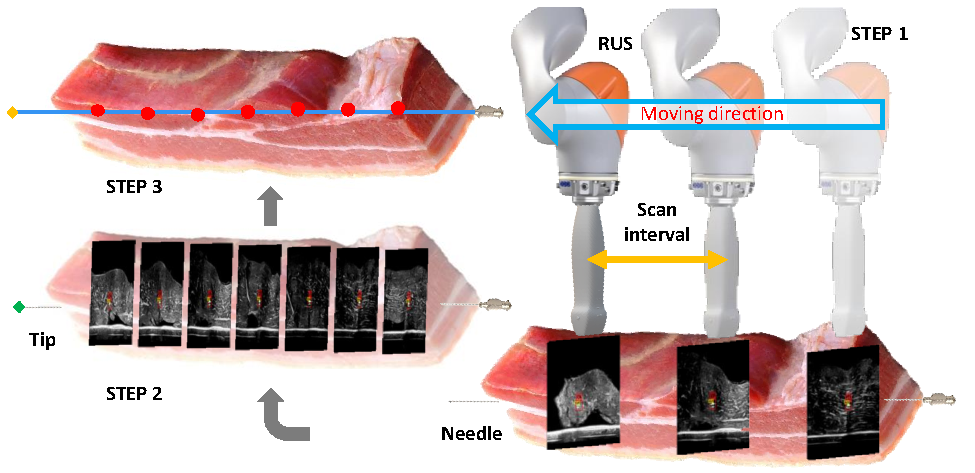
\includegraphics[width= 0.9\textwidth]{figures/2/f1.pdf}
\captionsetup{width=16 cm,justification=centering}
\caption{The proposed tip estimation method. STEP 1: 2D transverse US images with needle cross sections are collected by using RUS; STEP 2: Needle cross sections are detected and tracked in the successive US images; STEP 3: Needle shape is constructed and its tip is estimated.}\label{fig:1}
\end{figure}

In this paper, we present a method to track a long-curved needle from the 2D transverse US images and estimate its tip for the guidance of needle insertion.
Ultrasound is first used to detect the cross sections of the long-flexible needle (shown in Figure \ref{fig:1} STEP 1).
The needle shape tracking method combined needle detection with Kalman filter, develops an accurate location and a robust tracking procedure from 1 mm to 8 mm scan intervals (shown in Figure \ref{fig:1} STEP 2).
Unlike the previous study\cite{Waine2016a}, the 3D needle positions obtained from 2D US images and optical tracking system have been used in KF for the precise location.
Curve fitting method is then used to achieve the shape reconstruction and the needle tip position is estimated based on its length and the curve fitting result (shown in Figure \ref{fig:1} STEP 3).
The advantage of the proposed method is that the shape and tip position can be estimated through scanning the needle's cross sections at intervals along the direction of needle insertion without detecting the tip.
%The advantage of the proposed method is that the tip is estimated through scanning the needle's cross sections.
%Moreover, if the needle is deflected in the tissue, the tip position can be estimated accurately when the probe scans along the direction of needle insertion.
Besides, a novel histogram method is introduced to detect the needle in image processing, which can improve the needle localization under the effect of needle comet tail and the poor reflection, despite of the abrupt intensity changes.
In addition, a robotic ultrasound system (RUS)\cite{Priester2013} is built to evaluate the proposed needle tip estimation method. Results showed that the estimation of tip position is less than 1 mm within 4 mm scan intervals.

The rest of this paper is organized as follows. The proposed methods will be introduced in detail in Section II. Section III intends to represent the experimental setup and the results. Finally, discussion and conclusion will be drawn in the Section IV.



%%%%%%%%%%%%%%%%%%%%%%%%%%%%%%%%%%%%%%%%%%%%%%%%%%%%%%%%%%%%%%%
\section{Materials and Methods}

The proposed needle tip estimation method in successive transverse US images can be divided in three stages: needle detection, needle shape tracking and tip estimation. The processing diagram are shown in the Figure \ref{fig:2}. The needle location will be manually selected as an initial region of interest (ROI) by the binary method in the first US image. After that, the prediction of needle position from a Kalman Filter can be transformed in the transverse US images. At the same time, the next needle position in this ROI can be found through the histogram method. The KF is then updated for current precise needle position and prediction of the next position. After all the cross sections of needle have been collected, the needle shape can be fitted by curve fitting method (part C in Figure \ref{fig:2}). Finally, the position of the needle tip can be estimated from the curve fitting result based on the length of the needle. In this study, the ROI is set as a square window with the length of three times larger than the needle diameter and its center represents the needle position. Needle detection (part B in Figure \ref{fig:2}) is mainly about the image processing, while Kalman filter is used for needle shape tracking (part A in Figure \ref{fig:2}).

\begin{figure}[H]
\centering
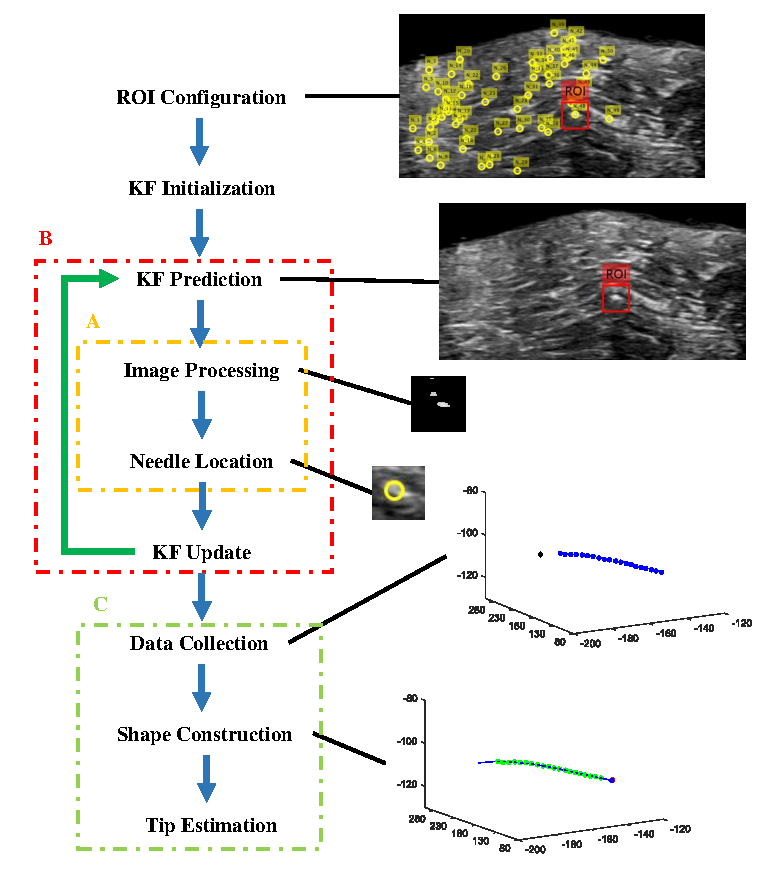
\includegraphics[width=0.8\textwidth]{figures/2/f2.pdf}
\captionsetup{width=16 cm,justification=centering}
\caption{ The pipeline of curved needle tip estimation. As the ROI configuration finished, needle tracking with needle detection begins step by step. Part A shows the needle tracking by KF, while Part B shows the needle detection to locate the needle tip. Part C shows the shape construction and tip estimation.}\label{fig:2}
\end{figure}

\subsection{Needle detection }
Needle detection is mainly for identifying the cross section of needle in the US images by the following methods: binary method and histogram method.
Since the ultrasound is quite sensitive to the metal, the needle-inside area can be brighter than others.
A binary method\cite{Waine2016a} is first used to select ROI in the first image and then a histogram method is used to locate the needle despite of US shadows and poor reflection.

Binary method intends to strengthen the contrast of brightness to highlight the brighter area in order to select them.
This method is used for the initialization which is supposed to find the candidates in the first image.
It includes intensity normalization, background reinforce and brightness enhancement.
And the center of the area is the location of the needle.
During the experiment, a histogram method is proposed to find the needle accurately.
The histogram method contains intensity normalization and background reinforce.
The histogram method tends to find an area of high intensity pixels, which intends to find the upper face of the needle and then locate needle based on the diameter.
The background reinforce part can be described as follows:
%\begin{equation}
%P_{I_k} = \frac{n_{I_k}}{M}
%\end{equation}
%\begin{equation}
%\mathop{\arg\min}_{t} \sum_{t}^{255} P_{I_k} \geq \delta
%\end{equation}
%where ${I_k}$ is the grey level of the pixel,and ${k\in[0,255]}$. ${P_{I_k}}$ is the percentage of ${I_k}$ pixel in grey level with the number ${n_{I_k}}$, M is the total number of the grey level pixel in the image, and t([0,255]) is the variable which ensures the sum of ${P_{I_k} \geq \delta}$, while ${\delta}$ is the percentage to limit the bright pixels. The equations can then be simplified by:
%\begin{equation}
%\mathop{\arg\min}_{t} \sum_{t}^{255} n_{r_k} \geq M\delta(=N)
%\end{equation}
%where N is the number to limit the bright area, and we set it to be 40.
%\begin{mini*}|s|
%{}{I_t}
%{}{}
%\addConstraint{\sum_{I_t}^{255} n_{I_k} \geq M\delta}
%\addConstraint{I_t\in[0,255]}{}
%\end{mini*}
\begin{equation}
\begin{aligned}
\textrm{min} \quad & \quad I_t \\
%\end{equation}
%\begin{equation}
\textrm{s.t.} \quad & \sum_{I_t}^{255} n_{I_j} \leq M\delta \\
 &I_t\in[0,255] \\
\end{aligned}
\end{equation}
where ${I_j}$ is the grey level of the pixel and ${n_{I_j}}$ is the number of pixels which have the grey level of ${I_j}$.
${M}$ is the size of ROI, and ${\delta}$ is the manually selected parameter to limit the bright pixels.
In this work, ${M}$ is the square of ${45\times45}$, and ${\delta}$ was set to 0.08 based on empirical tests.

\begin{figure}[H]
\centering
\subfigure[Elimination of Comet tail.]
{
\label{fig:3a}
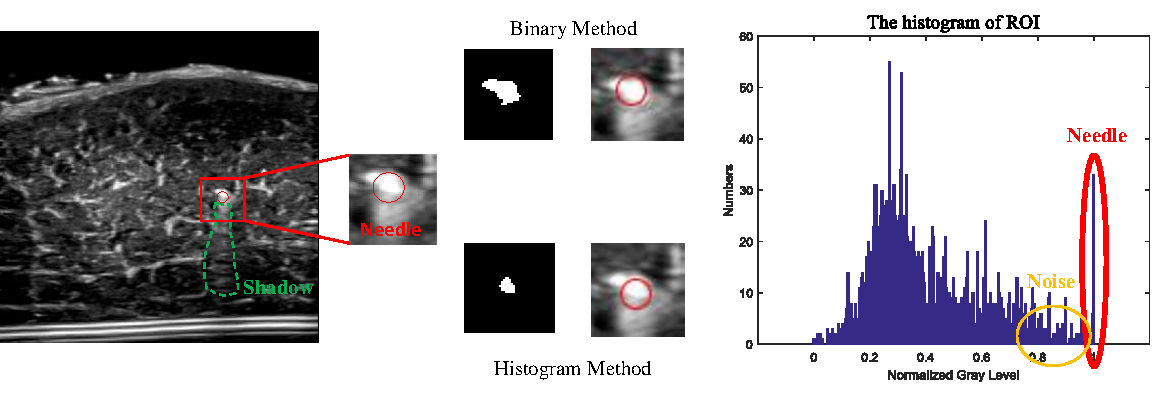
\includegraphics[width=\textwidth]{figures/2/f3a.pdf}
}
\subfigure[Poor reflection.] {
\label{fig:3b}
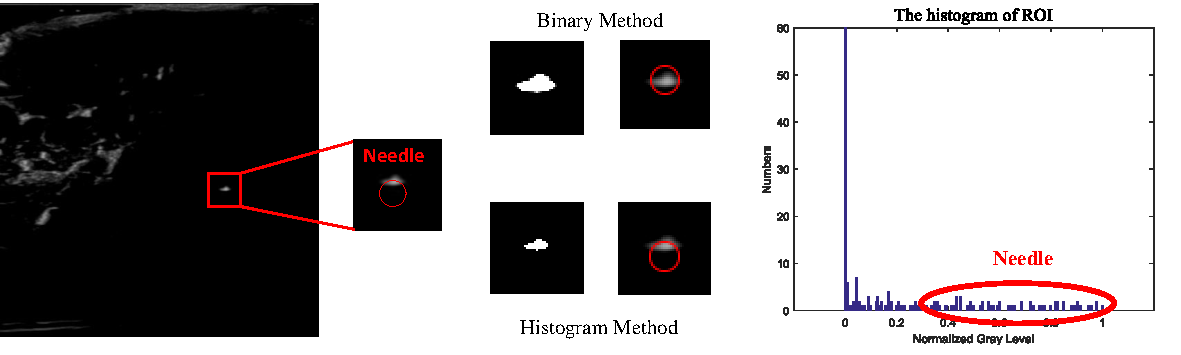
\includegraphics[width=\textwidth]{figures/2/f3b.pdf}
}
\captionsetup{width=16 cm,justification=centering}
\caption{Two cases may generate the errors: (a) the comet tail of needle with binary method process, histogram method process and the histogram of ROI; (b) the poor reflection of the needle with histogram method process and the histogram of ROI.}
\label{fig:3}
\end{figure}

%Although the binary method can detect the needle in most images,
There are two unexpected situations that may affect the position accuracy, namely the comet tail and the poor reflection.
The comet tail will affect the size of the needle area and usually obtain a larger area than actual size (Figure \ref{fig:3a}).
On the contrary, the poor reflection makes the needle area look much smaller in the image (Figure \ref{fig:3b}).
Therefore, the accurate location should be intended to eliminate the effect of shadows and poor reflection.
In Figure \ref{fig:3}, there are two examples which are used two methods relatively.
As the example shown in Figure \ref{fig:3a}, the noise (yellow circle in histogram of ROI) may probably be concerned as the needle while the needle is just concerned about few pixels (red circle in histogram of ROI).
And two methods can both filter the noise and locate the needle correctly.
But in ROI configuration (shown in Fig.\ref{fig:2}), the histogram method intends to find more candidates than the binary method, since the former focuses on the higher intensity pixels while the latter focuses on the area and intensity.
Therefore, the binary method is more feasible in ROI configuration.

However, in the case of poor reflection, the needle displays a little in the image, and the area of needle is smaller than the expected.
Because the needle would reflect as long as the image gain is high enough or the sound power is big enough, it would reveal apparently compared to its surroundings. Such like the histogram of ROI shown in Figure \ref{fig:3b}, the red circle represents the upper surface of the needle.
Moreover, ROI square is darker than the one in Fig.\ref{fig:3a}, while the settings of the ultrasound are the same in Fig.\ref{fig:3}.
From the figure, the histogram method seems to be more accurate than the binary method.
But in fact, the error of two methods in this case is 0.34 mm with 1.2 mm diameter of needle.
It is not that obvious to judge the accuracy.
In this study, we use the histogram method during the experiment.

\subsection{Needle shape tracking}

As indicated in previous researches \cite{Mignon2018,Mignon2016,Yue2012}, Kalman filter has been successfully used for tracking needle in the successive ultrasound images.
In this study, Kalman filter is used to improve the estimation of the needle location in successive frames.
As shown in Fig.\ref{fig:4}, the applied Kalman filter has two process, prediction and update.
The prediction stage intends to locate the needle position previously, and set the ROI (Red and yellow square in Fig.\ref{fig:4}) in order to find the needle precisely with small window which is supposed to reduce the computation.
The update stage is the result of needle position after the measurement from histogram method.

\begin{figure}[H]
\centering
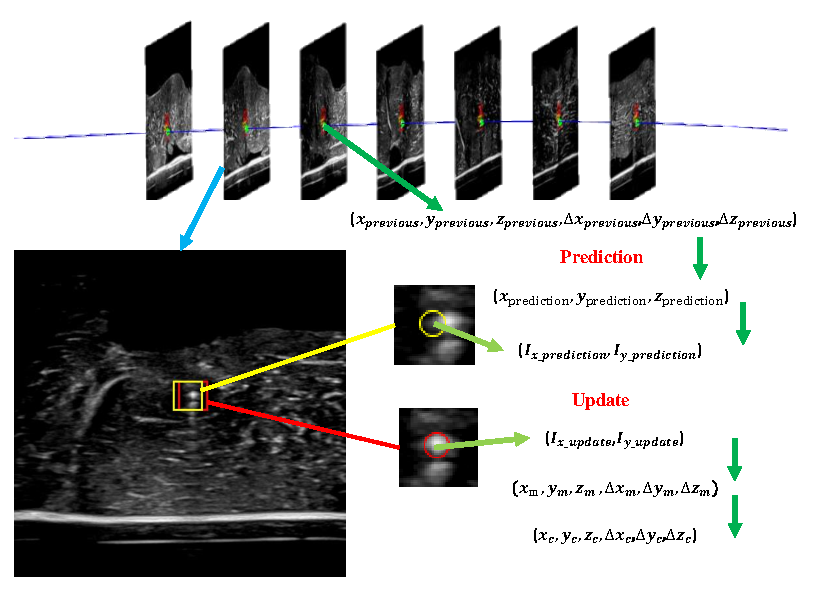
\includegraphics[width=0.8\textwidth]{figures/2/f4_g1.pdf}
\captionsetup{width=16 cm,justification=centering}
\caption{
Two steps of Kalman Filter.
As the next US image is acquired, the previous state ${(x_{previous},y_{previous},z_{previous},\triangle x_{previous},\triangle y_{previous},\triangle z_{previous})}$ is used to predict the needle position ${(x_{prediction},y_{prediction},z_{prediction}}$, which then will be transformed to ${(I_{x\_prediction},I_{y\_prediction})}$ in the image as the center of ROI.
The yellow square is the ROI corresponding to ${(I_{x\_prediction},I_{y\_prediction})}$ and the red one is the update step in KF by using the measurement data from needle detection to locate the needle with its center ${(I_{x\_update},I_{y\_update})}$ as the needle position.
Finally, the measurement state ${(x_{m},y_{m},z_{m}, \triangle x_{m},\triangle y_{m},\triangle z_{m})}$ and the current state ${(x_{c},y_{c},z_{c}, \triangle x_{c},\triangle y_{c},\triangle z_{c})}$ can be obtained.
}\label{fig:4}
\end{figure}

The state prediction ${\hat{t}_i}$ intends to represent the prediction state of the transverse needle center position ${(x, y, z)}$ in the reference frame with the change of the needle position ${(\triangle x,\triangle y,\triangle z)}$ at sample ${i}$ according to the state t. ${(\triangle x,\triangle y,\triangle z)}$ are the difference between the previous needle position and the current needle position. ${t_i}$ is the result from the previous iteration which is as follows:
\begin{equation}
t_i =
\begin{bmatrix}
x_i\\
y_i\\
z_i\\
\triangle x_i\\
\triangle y_i\\
\triangle z_i
\end{bmatrix}
\end{equation}
%For the controlled variable of the robot arm, it can be considered as the movement of the marker bound on the robot arm. Therefore, the controlled variable can be equivalent to ${\tilde{u}_k}$, which is the difference of two adjacent positions of the marker, displayed as:
%\begin{equation}
%Bu_k = \tilde{u}_k
%\end{equation}
Where ${\triangle x_1}$ and ${\triangle y_1}$ are set to be 0, while ${\triangle z_1}$ is equal to the scan interval.
Then, the prediction equations are as follows:
\begin{equation}
\hat{t}_i= At_{i-1}
\end{equation}
\begin{equation}
\hat{P}_i=AP_{i-1}A^T+Q
\end{equation}
The measurement update equations are as follows:
\begin{equation}
K_i=\hat{P}_iH^T(H\hat{P}_iH^T+R)^{-1}
\end{equation}
\begin{equation}
\label{eq:6}
t_i=\hat{t}_i+K_i(m_i-H\hat{t}_i)
\end{equation}
\begin{equation}
P_i=(I- K_iH)\hat{P}_i
\end{equation}
Where A, H, R and Q are:
\begin{equation}
A =
\begin{bmatrix}
1 \quad 0 \quad 0 \quad 1 \quad 0 \quad 0\\
0 \quad 1 \quad 0 \quad 0 \quad 1 \quad 0\\
0 \quad 0 \quad 1 \quad 0 \quad 0 \quad 1\\
0 \quad 0 \quad 0 \quad 1 \quad 0 \quad 0\\
0 \quad 0 \quad 0 \quad 0 \quad 1 \quad 0\\
0 \quad 0 \quad 0 \quad 0 \quad 0 \quad 1\\
\end{bmatrix}
\end{equation}
\begin{equation}
H=
\begin{bmatrix}
I_{6\times6}
\end{bmatrix}
,R=Q=10^{-6}\times
\begin{bmatrix}
I_{6\times6}
\end{bmatrix}
\end{equation}
A is the state transition matrix, H is the measurement matrix. ${\hat{P}_i}$, ${P_i}$ are the priori and posteriori estimate error covariance, and R, Q are the measurement error covariance and processing error covariance respectively.
${K_i}$ is the Kalman gain at sample i.
${m_i}$ is the measurement state from the needle detection.

The prediction 3D position ${(x_{prediction},y_{prediction},z_{prediction})}$ is obtained from the previous state.
And before the needle detection in the current US image, this should be transformed on the image plane frame as 2D position ${(I_{x\_prediction},I_{y\_prediction})}$.
Then, after update, the needle position ${(I_{x\_update},I_{y\_update})}$ in the image will be transformed to ${(x_{m},y_{m},z_{m})}$, back to the 3D position.
And also, we can get ${(\triangle x_{m},\triangle y_{m},\triangle z_{m})}$from:
\begin{equation}\label{eq:15}
\begin{aligned}
(\triangle x_{m},\triangle y_{m},\triangle z_{m})=(x_{m},y_{m},z_{m})-(x_{previous},y_{previous},z_{previous})
\end{aligned}
\end{equation}
Then, the measurement state ${m_i}$ in this frame is acquired as${(x_{m},y_{m},z_{m},\triangle x_{m},\triangle y_{m},\triangle z_{m})}$.
Through the measurement update, the current state can be obtained as ${(x_{c},y_{c},z_{c},\triangle x_{c},\triangle y_{c},\triangle z_{c})}$ from \ref{eq:6}.
The relationship between these transformations will be described in the next subsection.
In the previous study \cite{Waine2016a}, the data from the image has only two dimensions, lacking the data from the direction along the movement of the probe, which leads to the incomplete location.
Moreover, the space information is more capable to locate the needle accurately than the plane information.
Therefore, 3D positions have been used in the KF for the precise location.
The KF in this work is not only used for filtering, but also for predicting the next needle position in the US image.
And the ROI for the next iteration is centered around the needle position of the Kalman Filtering prediction, helping remove the outliers from the ROI.

\subsection{Tip estimation}
Before tip estimation, 2D points should be transformed to 3D points based on the relationship of each frames. The relationship among the reference frame, probe frame, marker frame and image frame are specified in Figure \ref{fig:5}.

\begin{figure}[H]
\centering
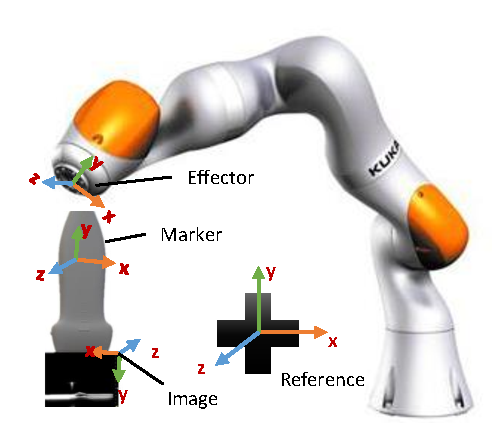
\includegraphics[width=8.2 cm]{figures/2/f5.pdf}
\captionsetup{width=16 cm,justification=centering}
\caption{The relationship of the frames.}\label{fig:5}
\end{figure}

As shown in Figure \ref{fig:5}, the image has one plane with 2 axis (axis x and axis y) and axis z is vertical to the image. Moreover, the probe has the completely same frame with image, except that the probe frame is designed in millimeters and the image frame is set in pixels. Equation (9) implies the transformation from image to reference:
\begin{equation}
{Point}_1=T_{marker}^{ref}\times T_{probe}^{marker}\times T_{image}^{probe}\times {Point}_2
\end{equation}
Where ${{Point}_1}$ and ${{Point}_2}$ are the points on the reference frame and image frame respectively, ${T_{marker}^{ref}}$ is the transformation from reference frame to the marker frame, ${T_{probe}^{marker}}$ is the transformation from the marker frame to the probe frame, ${T_{image}^{probe}}$ is the transformation from the probe frame to the image frame. Through this transformation, the needle position in the image can be directly re-defined in the reference frame for the needle tracking and curve fitting.

The tip estimation has two steps: curve fitting and tip estimation. It has been shown that the cubic line model can be used to estimate the needle. In this study, third-order curve line is used for the shape construction where the equations can be written as:
\begin{equation}
f(x)=\sum_{k=0}^{3}a_k x^k
\end{equation}
\begin{equation}
g(x)=\sum_{k=0}^{3}b_k x^k
\end{equation}
Where ${f(x)}$ and ${g(x)}$ are the equations to fit the line along the x, which is the axis with the same direction of the insertion. ${(a_0,a_1,a_2,a_3)}$ and ${(b_0,b_1,b_2,b_3)}$ are the free parameters of the needle shape model.

After sample points of the inflected needle have been obtained, least square curve fitting method will be used to fit these points as a cubic line. The target functions to fit the cubic line can be defined as follows:
\begin{equation}
F(a_0,a_1,a_2,a_3)=\min\sum_{i=1}^{n}(f(x_i)-y_i)^2 =\min\sum_{i=1}^{n}(\sum_{k=0}^{3}a_k x_i^k-y_i)^2
\end{equation}
\begin{equation}
G(b_0,b_1,b_2,b_3)=\min\sum_{i=1}^{n}(g(x_i)-z_i)^2 =\min\sum_{i=1}^{n}(\sum_{k=0}^{3}b_k x_i^k-z_i)^2
\end{equation}
where n is the number of the points ${(n\geq4)}$ and ${(x_i,y_i,z_i)}$ is the position of point ${i}$. By applying the ${l_2}$ norm minimization in the two dimensional Euclidean space, it can be formulated as:
\begin{equation}
\mathop{\arg\min}_{t\in R} {\|X{\textbf{\textit{a}}}-Y\|}_2
\end{equation}
where ${{\textbf{\textit{a}}}=[a_0,a_1,a_2,a_3]'}$, ${Y=[y_1,y_2,\ldots,y_n]'}$ and ${X}$ can be written as:
\begin{equation}
X= \begin{bmatrix}
1&x_1&{x_1}^2&{x_1}^3\\
1&x_2&{x_2}^2&{x_2}^3\\
\vdots&\vdots&\vdots&\vdots\\
1&x_n&{x_n}^2&{x_n}^3
\end{bmatrix}
\end{equation}

The solution can be estimated as follows:
\begin{equation}
{\textbf{\textit{a}}}={(X^T X)}^{-1} X^T  Y
\end{equation}
From this solution, ${f(x)}$ and ${g(x)}$ can be obtained to construct needle shape. The tip position can then be estimated by the following optimum solutions based on the length of the needle:
\begin{equation}
\centering
\begin{aligned}
\textrm{min} \quad & \|\int_{{tail}_x}^{{tip}_x}\sqrt{1+{\acute{f(x)}}^2+{\acute{g(x)}}^2 }dx-L\|_2\\
%\end{equation}
%\begin{equation}
\textrm{s.t.} \quad & {tip}_x>{tail}_x \\
\end{aligned}
\end{equation}

%\begin{equation}
%\begin{aligned}
%F({tip}_x )&=\int_{{tail}_x}^{{tip}_x}\sqrt{1+{\acute{f(x)}}^2+{\acute{g(x)}}^2 }dx-L \\
%&=\int_{{tail}_x}^{{tip}_x}\sqrt{1+(a_1+2a_2 x+3a_3 x^2)^2+(b_1+2b_2 x+3b_3 x^2)^2 }dx-L
%\end{aligned}
%\end{equation}
where ${{tail}_x}$ is the measured value of tail position from optical tracker, ${{tip}_x}$ is the expected value of the tip position in axis ${x}$, ${L}$ is the length of the needle.

%%%%%%%%%%%%%%%%%%%%%%%%%%%%%%%%%%%%%%%%%%
\section{Results}
\subsection{Experimental Platform Setup}
To verify the proposed tip tracking and shape sensing method, the robotic ultrasound system has been built, which includes a KUKA IIWA robot arm, a Wisonic ultrasound scanner, an NDI optical tracker, an NDI electromagnetic (EM) tracker and a computer. As shown in Figure \ref{fig:6}, the US probe is mounted on the effector of robot arm by the gripper attached to the passive marker. The phantom or ex-vivo (like chicken breast in Figure \ref{fig:6}) is punctured by an 18G beveled-tip needle with 200 mm long, while the needle tip is completely exposed for validation.
The diameter of the needle is 15 pixels in image.
The NDI optical tracker is used for localize the marker bound with probe, while NDI electromagnetic tracker is used for validate the tip position.

Experiments have been taken in a water tank, which provides a liquid environment for the ultrasound.
And the needle is placed in water or inserted in the silica gel phantom (shown in \ref{fig:002a}), pork and chicken breast.
The depth of the ultrasound is set to 4 cm.
And in this study, the needle is usually detected in 1 to 3 cm from the US probe.
During the experiment, the robot arm automatically moves with ultrasound probe along the direction of the needle insertion, but does not have any contact with the tissue (shown in \ref{fig:002b}).
The whole scan length is at most 160 mm which depends on the scan intervals (shown in table 1). The scan interval decreases with the increasing collected points.

\begin{table}[H]
\caption{Scan lengths with different scan intervals.}
\centering
%% \tablesize{} %% You can specify the fontsize here, e.g., \tablesize{\footnotesize}. If commented out \small will be used.
\begin{tabular}{ccc}
%\toprule
\rowcolor{gray!40}\textbf{Scan Interval}  & \textbf{Scan Length}  & \textbf{Points}\\
%\midrule
\hline 1 mm    & 160 mm    & 160\\
\hline 2 mm    & 159 mm    & 80\\
\hline 3 mm    & 160 mm    & 54\\
\hline 4 mm    & 157 mm    & 40\\
\hline 5 mm    & 156 mm    & 32\\
\hline 6 mm    & 157 mm    & 27\\
\hline 7 mm    & 155 mm    & 23\\
\hline 8 mm    & 153 mm    & 20\\
\bottomrule
\end{tabular}
\end{table}

\begin{figure}[H]
\centering
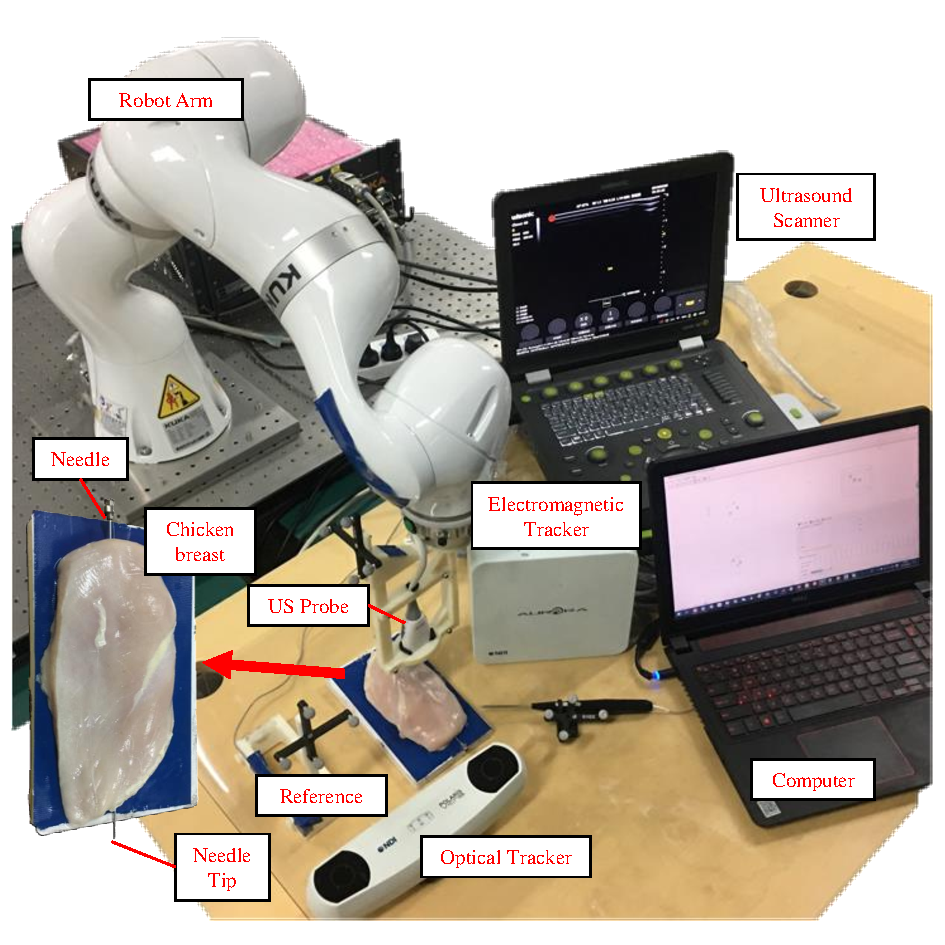
\includegraphics[width=0.9\textwidth]{figures/2/f6.pdf}
\captionsetup{width=16 cm,justification=centering}
\caption{The devices of the experiment.}\label{fig:6}
\end{figure}

Before data collection, the US image and the marker need to be calibrated. After that, the experiment starts after the needle finished puncturing manually. Robot arm is used to move the US probe scanning along the needle. Meanwhile, pose data are collected from the optical tracker and US images from the Ultrasound scanner. Finally, the tail of the needle and its tip are measured by the optical and electromagnetic sensors respectively for the curve fitting and the tip validation. The needle is inserted manually, imitating the real situations of percutaneous interventions.

\begin{figure}[H]
\setlength{\subfigcapskip}{-1bp}
\centering
\begin{minipage}{\textwidth}
\centering
\subfigure{\label{fig:002a}}\addtocounter{subfigure}{-1}
\subfigure[Phantom with inserted needle]{
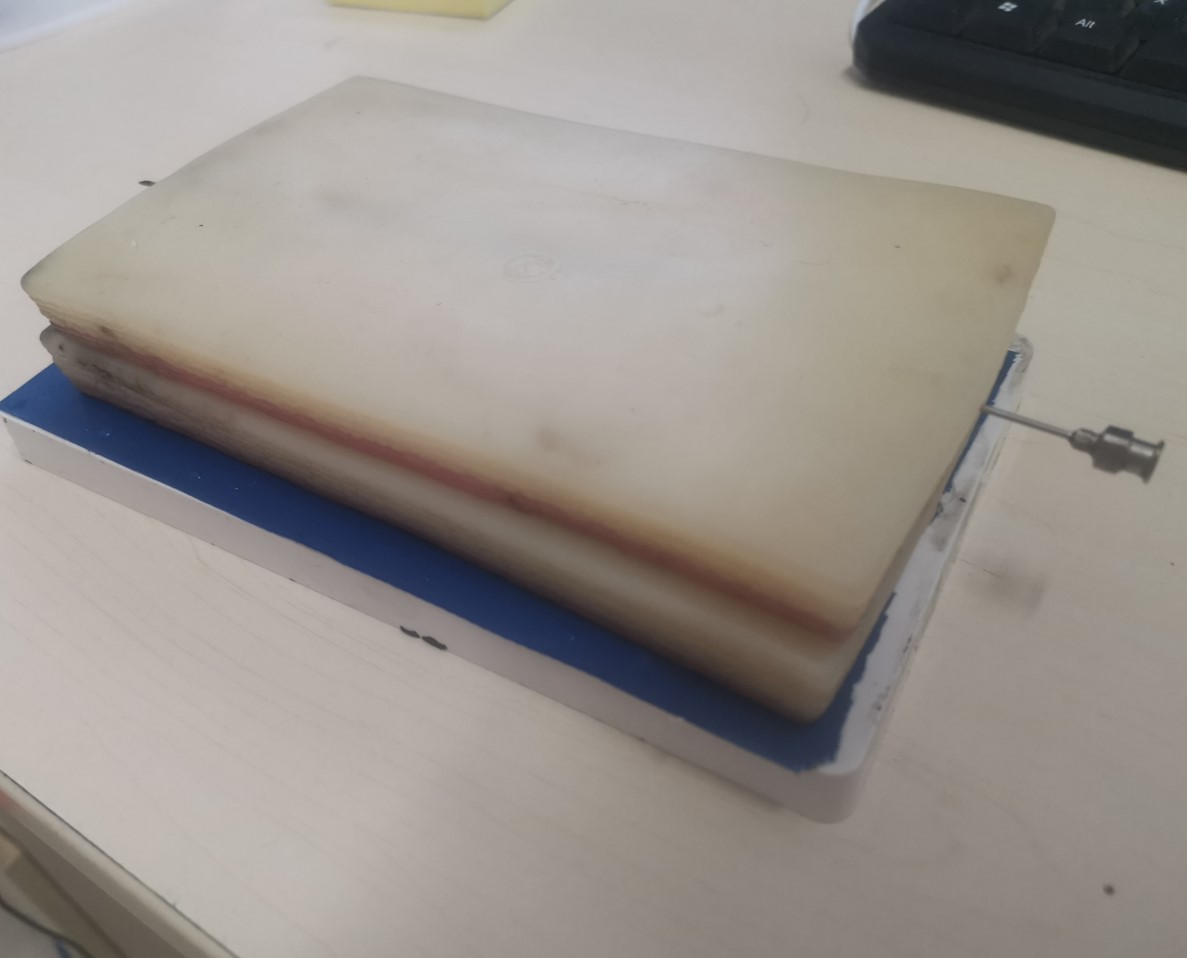
\includegraphics[width=0.4\textwidth]{figures/2/fz_2a.jpg}}
\hspace{2em}
\subfigure{\label{fig:002b}}\addtocounter{subfigure}{-1}
\subfigure[The probe scans without any contact]{
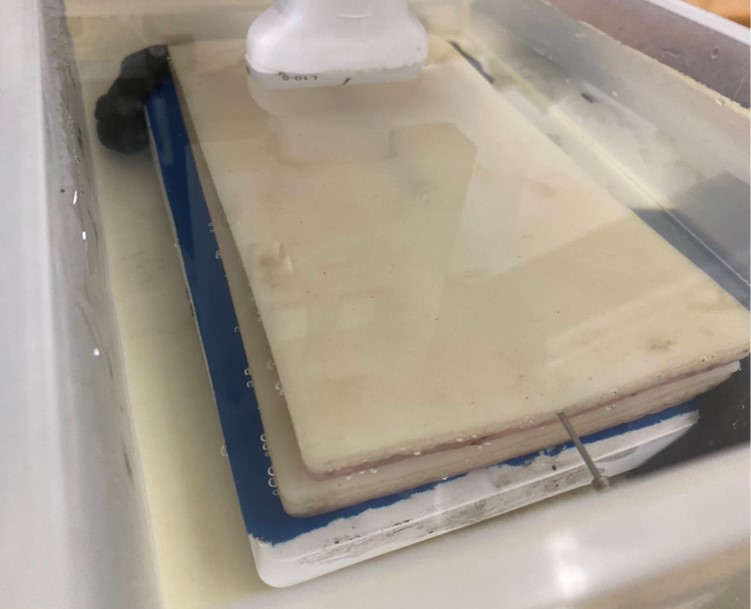
\includegraphics[width=0.4\textwidth]{figures/2/fz_2b.jpg}}
\end{minipage}
\vspace{0.1em}
\caption[The phantom used in the experiment and the movement of the probe.]{The phantom used in the experiment and the movement of the probe.}\label{fig:002}
\end{figure}

\subsection{Tip estimation}
Four kinds of platforms have been used in the experiments, water, phantom, chicken, and pork. Each platform has been tested several times. Figure \ref{fig:7} shows one test in chicken breast. In this case, the US probe moved along the needle in the chicken breast every 4 mm. The black square point on the left is the needle tail position and the blue line is the estimated needle shape. The green points are the detected needle and considered as the center of the needle, the blue point is the estimated tip position and the red point is measured tip position from EM. The estimation error is 0.69 mm in this test.
\begin{figure}[H]
\centering
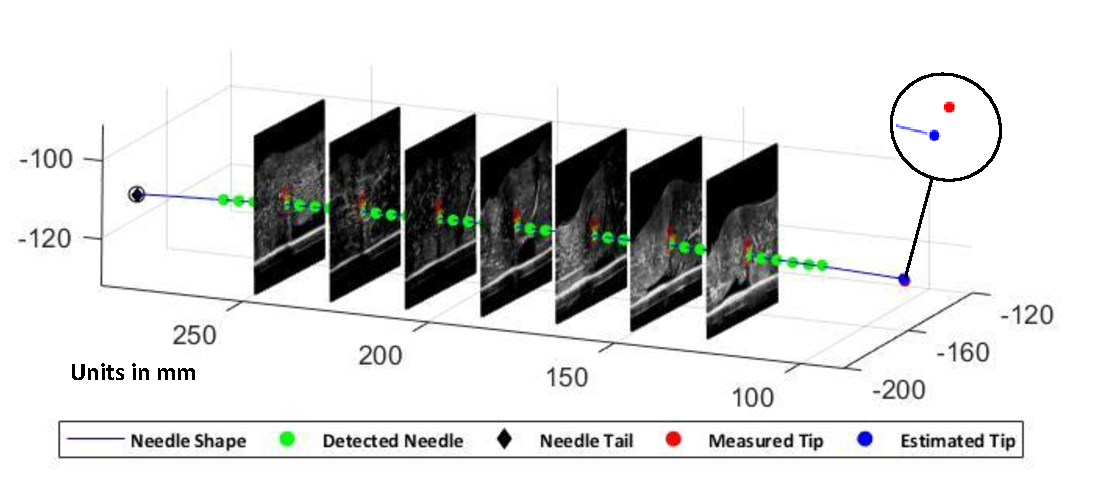
\includegraphics[width=\textwidth]{figures/2/f7.pdf}
\captionsetup{width=14 cm,justification=centering}
\caption{Experiment in chicken breast with 4 mm scan interval.}\label{fig:7}
\end{figure}

The error of the algorithm is shown in table 2, which suggests that the errors increase with the increase of scan intervals. Figure \ref{fig:8} shows the results of the experiment on four platforms. The mean errors are all under 0.4 mm with 1 mm scan interval in the four experiments, while the error is around 1 mm with 8 mm.

\begin{figure}[H]
\setlength{\subfigcapskip}{-1bp}
\centering
\begin{minipage}{\textwidth}
\centering
\subfigure{\label{fig:8a}}\addtocounter{subfigure}{-1}
    \subfigure[The Experiments in Water.]{
    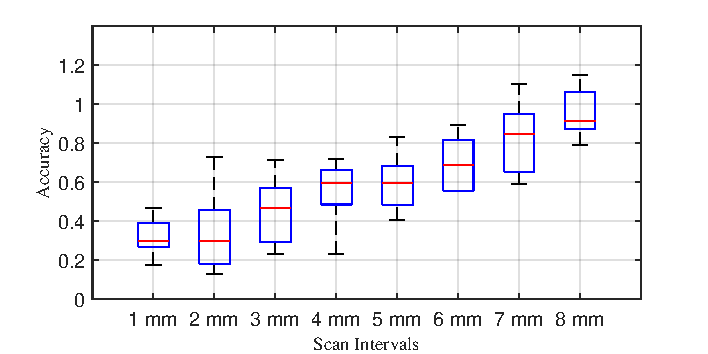
\includegraphics[width=0.4\textwidth]{figures/2/f8a.pdf}
    }
\hspace{1em}
\subfigure{\label{fig:8b}}\addtocounter{subfigure}{-1}
    \subfigure[The Experiments in Phantom.]{
    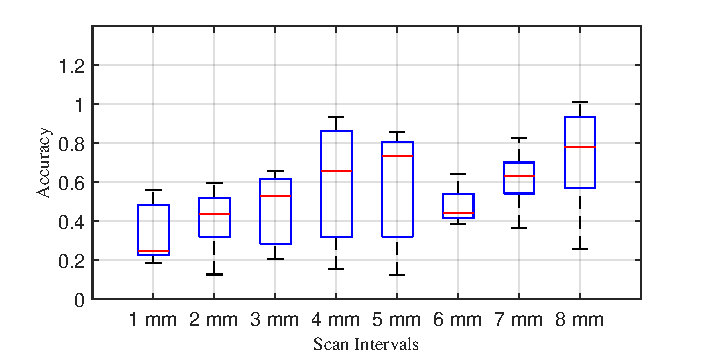
\includegraphics[width=0.4\textwidth]{figures/2/f8b.pdf}
    }
\end{minipage}
\centering
\begin{minipage}{\textwidth}
\centering
\subfigure{\label{fig:8c}}\addtocounter{subfigure}{+1}
    \subfigure[The Experiments in Pork.]{
    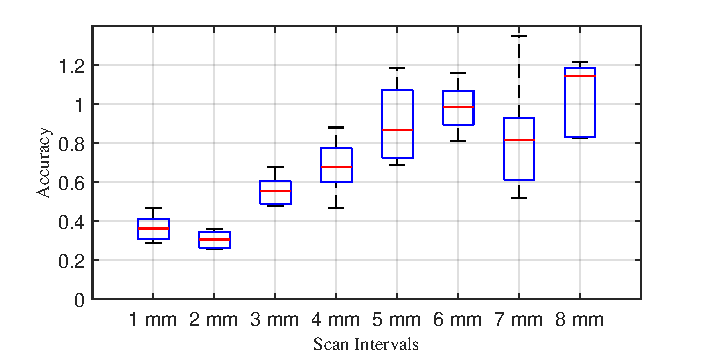
\includegraphics[width=0.4\textwidth]{figures/2/f8c.pdf}
    }
\hspace{1em}
\subfigure{\label{fig:8d}}\addtocounter{subfigure}{-1}
    \subfigure[The Experiments in Chicken.]{
    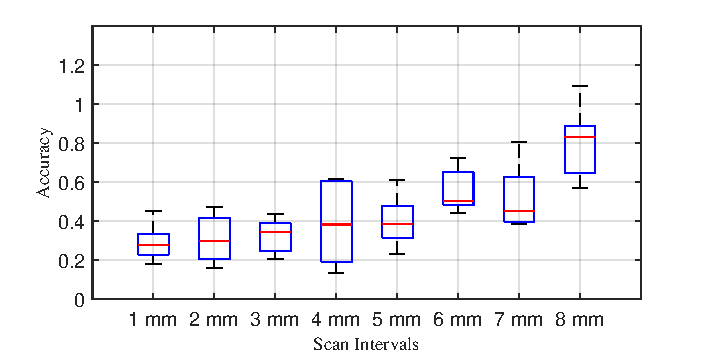
\includegraphics[width=0.4\textwidth]{figures/2/f8d.pdf}
    }
\end{minipage}
\caption{The experiment with different scan intervals on four platform.}\label{fig:8}
\end{figure}

\begin{table}[H]
\caption{The Results of Tip Estimation (mm).}
\centering
\begin{tabular}{p{2cm}<{\centering}|p{2cm}<{\centering}|p{2cm}<{\centering}|p{2cm}<{\centering}|p{2cm}<{\centering}}
%\toprule
\rowcolor{gray!70} \multicolumn{5}{c}{\textbf{Accuracy}}\\
\hline \rowcolor{gray!50}\textbf{Intervals}  & \textbf{Water}  & \textbf{Phantom}   & \textbf{Pork}   & \textbf{Chicken}\\
%\midrule
 1 mm   &${0.32\pm0.10}$   &${0.33\pm0.15}$    &${0.37\pm0.07}$    &${0.29\pm0.09}$\\
2 mm   &${0.36\pm0.21}$   &${0.41\pm0.16}$    &${0.31\pm0.05}$    &${0.31\pm0.12}$\\
3 mm   &${0.45\pm0.16}$   &${0.46\pm0.18}$    &${0.56\pm0.08}$    &${0.33\pm0.09}$\\
4 mm	&${0.55\pm0.16}$	&${0.59\pm0.31}$	&${0.68\pm0.14}$	&${0.38\pm0.21}$\\
5 mm	&${0.60\pm0.13}$	&${0.59\pm0.29}$	&${0.90\pm0.20}$	&${0.40\pm0.14}$\\
6 mm	&${0.69\pm0.13}$	&${0.48\pm0.09}$	&${0.99\pm0.13}$	&${0.55\pm0.11}$\\
7 mm	&${0.83\pm0.17}$	&${0.62\pm0.14}$	&${0.84\pm0.30}$	&${0.52\pm0.17}$\\
8 mm	&${0.95\pm0.11}$	&${0.73\pm0.26}$	&${1.06\pm0.18}$	&${0.81\pm0.19}$\\
\bottomrule
\end{tabular}
\end{table}

\section{Discussion \& Conclusion}
Needle insertion guided by ultrasound images is widely used for percutaneous interventions. However, the needle detection due to its deflection by the inevitable factors is challenging during the needle insertion. Such factors include needle-tissue interaction, improper insertion force, physiological motions, and so on. Automatic needle detection with needle tracking in 2D transverse US images could overcome these limitations and estimate needle tip through the curve-fitting method. The target of this study was to develop a robust needle detection and tracking method with the help of ultrasound images to estimate the needle tip precisely and accurately. We used a histogram method to detect the needle in transverse US images to decrease the effects of comet tail and poor reflection. In a subsequent post-processing, the needle was tracked by Kalman filter tracking method in consecutive US images with the help of the displacement of the probe. A third-order curve fitting method has been used to estimate the needle tip. When the probe is moved by the robot arm, the scanning time is different. We assume that the time when the probe stops to collect the data is the same. The less scan interval we choose, the more collection points we can obtain and the more scanning time it takes. Therefore, the scanning time mainly depends on the quantity of scanning points while the accuracy lies on how short the scan interval is. In other words, the accuracy of the tip estimation can be improved by reducing the scan interval to collect more needle positions. However, this will consume more scanning time and reduce the efficiency of tracking. Inversely, fewer collecting positions would cost less time but may lead to a more possibility of the failure of shape construction and a more possibility of large error of the tip estimation. As a result, how to balance precision and scanning time is very important to make the proposed method more efficient. In our experiment, it is found that 4 mm scan interval has an error less than 1 mm, which is a better choice to satisfy both requirements.

In the proposed method, needle shape tracking has a great contribution to the accurate localization, since the needle can be tracked precisely by Kalman filter through its prediction and update. However, needle shape tracking is heavily dependent on the scan interval, especially for a strongly curved needle, since Kalman filter is generally well functioned in the lineal system. As a result, if the needle is deflected during insertion, the Kalman filter would make mistakes and wrongly predict the needle position when the scan interval is large. In this study it is found that Kalman filter would fail if the scan interval is more than 8 mm. This may due to the impact on the prediction of KF with a large deviation. Moreover, the deviation won’t be eliminated even with change of ROI size. Besides, Histogram methods showed the accurate and effective detection of the needle, but it relies on the brightness of the image since the needle could not be easily detected where there are plenty of pixels with the highest intensity (which is max value 255). However, this condition can be controlled by the setting of the ultrasound scanner to expand the grey level of the image properly.

This method still has its limitations.
During the experiment, the time is needed for the data collection from US scanner and optical tracking system, and the movement of the robot arm, which is affected by the scan length and scan interval.
However, it is very hard to acquire the whole positions of a long needle in one scan for any medical image sensor.
Therefore, in the future, it is valuable to find a method to reduce the times of needle detection in order to reduce the time for the tip estimation.
Moreover, when the robot arm moves with the US probe precisely, the tissue and needle have a possibility to be deformed by the probe motion.
Hence, it is necessary to make the robot arm move smoothly as well as correctly on the surface of tissue.
In addition, the patient motion is the biggest uncertain problem, which leads to the failure of needle insertion and detection.

In this system, we use 2D US scanner for the detection of needle in various kinds of tissue.
However, 3D US scanner can also be used in this system.
Although it has volume data and the detection method is different, the tracking method is able to be similar, since we also use the 3D positions for tracking in this study.
Moreover, the time is also needed for data collection and the movement of robot arm, especially for the long needle, which is easily out of view-field of US volumes or images.
Therefore, we use 2D US images in this study.

In this paper, a method for tracking a long-curved needle from the 2D transverse US images and the tip estimation is represented and demonstrated with RUS.
Ultrasound is first used to detect the cross section, with the probe moving along a long-flexible needle.
And then, the needle shape tracking method combined needle detection with Kalman filter by using 3D needle positions develops an accurate location and a robust tracking procedure.
Then, the needle shape is constructed by using curve fitting method and its tip position is estimated based on the former result.
A histogram method is introduced to detect the needle in image processing, which can improve the needle localization despite of the abrupt intensity changes.
This new imaging approach is proposed based on the selection of numbers of pixels with higher gray level, which can directly remove the lower gray level to highlight the needle.
The results of the experiments suggest that the detection of the needle by the histogram method and Kalman Filter has high precision with minimum error 0.13 mm with 1 mm scan interval in phantom experiment and maximum error 1.35 mm with 8 mm scan interval in pork experiment.
With the increase of the scan interval, the mean error would rise. And also, results showed that the estimation of tip position is less than 1 mm within 4 mm scan intervals.
We suggest to choose 4 mm scan interval to balance the precision and scanning time to maximize the efficiency.
%The scan length seems to influence the accuracy with the fact that the errors of the estimation in 7 mm (155 mm) and 8 mm (153 mm) scan intervals are commonly higher than the errors of other estimations.
In the future, we would make the experiments of how long the scan length is the best length to estimate the needle tip. The proposed method would be great assist to surgeons to locate the needle tip when they perform percutaneous insertion procedures with a long flexible needle, such as prostate brachytherapy.

\vspace{6pt}

\authorcontributions{Conceptualization,M.Q.H.M.; Validation, Z.L.;Writing-original draft,Z.L.;Writing-review and editing, S.S. and L.L.}

%%%%%%%%%%%%%%%%%%%%%%%%%%%%%%%%%%%%%%%%%%
\funding{This research was funded in part by the National Natural Science Foundation of China, grant number 61803123, and in part by  National Key R\&D Program of China, grant number 2018YFB1307700, and in part by Natural Science Foundation of Guangdong Province, China, grant number 2018A030310565.}

%%%%%%%%%%%%%%%%%%%%%%%%%%%%%%%%%%%%%%%%%%
\acknowledgments{For this kind of study, no formal ethics approval is required by the institutional ethics com. Informed consent was obtained from all individual participants included in the study.}

%%%%%%%%%%%%%%%%%%%%%%%%%%%%%%%%%%%%%%%%%%
\conflictsofinterest{The authors declare no conflict of interest.}

%%%%%%%%%%%%%%%%%%%%%%%%%%%%%%%%%%%%%%%%%%
%% optional
\abbreviations{The following abbreviations are used in this manuscript:\\

\noindent
\begin{tabular}{@{}ll}
KF & Kalman Filter\\
US & Ultrasound\\
RUS & Robot Ultrasound system\\
CT  & Computed Tomography\\
MRI  & Magnetic Resonance Imaging\\
RANSAC  & Random Sample Consensus
\end{tabular}}

% \reftitle{References}
% \bibstyle{plain}
% \bibliography{r1}
\externalbibliography{yes}
\bibliography{r1}

\end{document}
